% Two kinds of AI in research math. Ziff Davis, 2026-09-30.
% Build: ./slides/build.sh (tectonic). Sources for every Part 1 claim are in
% docs/navier-stokes-notes.md; Part 2 numbers are in docs/demo-outline.md.
\documentclass[aspectratio=169, 10pt]{beamer}
\usetheme[progressbar=frametitle, numbering=fraction, block=fill]{metropolis}
\usepackage{appendixnumberbeamer}
\usepackage{booktabs}
\usepackage{graphicx}
\usepackage{tikz}
\usetikzlibrary{arrows.meta, calc}

% Palette shared with src/pdes_demo/plotting.py: blue = interface-aware,
% orange = naive, neutral inks for everything else.
\definecolor{surface}{HTML}{FCFCFB}
\definecolor{ink}{HTML}{0B0B0B}
\definecolor{inksec}{HTML}{52514E}
\definecolor{inkmuted}{HTML}{8A8985}
\definecolor{layer}{HTML}{F0EFEC}
\definecolor{aware}{HTML}{2A78D6}
\definecolor{naive}{HTML}{EB6834}
\definecolor{navy}{HTML}{0D366B}

\setbeamercolor{normal text}{fg=ink, bg=surface}
\setbeamercolor{frametitle}{fg=surface, bg=navy}
\setbeamercolor{progress bar}{fg=aware, bg=layer}
\setbeamercolor{title separator}{fg=aware}
\setbeamercolor{alerted text}{fg=naive}
\setbeamercolor{example text}{fg=aware}
\setbeamercolor{block title}{fg=navy, bg=layer}
\setbeamercolor{block body}{fg=ink, bg=layer}
\setbeamercolor{footnote}{fg=inksec}

\hypersetup{colorlinks=true, urlcolor=aware, linkcolor=ink}

% Avenir Next on macOS, Latin Modern Sans elsewhere.
\IfFontExistsTF{Avenir Next}{\setsansfont{Avenir Next}}{}

\newcommand{\src}[1]{{\par\vspace{2pt}\scriptsize\color{inkmuted}#1\par}}
\newcommand{\clipnote}[2]{%
  \vspace{6pt}\begin{flushleft}\small\color{inksec}%
  \textbf{Play clip:} \texttt{#1} (#2)\end{flushleft}}
\newcommand{\q}[1]{``#1''}

\title{Two kinds of AI in research math}
\subtitle{A Millennium Prize claim, and an afternoon with a coding assistant}
\author{Brad Martin}
\date{30 September 2026}

\begin{document}

\maketitle

\begin{frame}{Why this talk}
  \begin{itemize}
    \item On 8 September, OpenAI said its AI had settled a 90-year-old,
      \$1M question about how fluids move.
    \item The night before, a mathematician and a coding assistant went
      public with a year of closely related work.
    \item Two weeks ago I rebuilt the simulation methods from my 2016
      dissertation with Claude Code, in a day.
  \end{itemize}
  \begin{block}{Thesis}
    \q{AI in research math} currently means two very different things.
    Both are worth seeing up close.
  \end{block}
  \begin{columns}[t]
    \column{0.48\textwidth}
      \textbf{Part 1 (15 min).} The Navier--Stokes claim: what was claimed,
      how it was produced, who else was there, what is still open.
    \column{0.48\textwidth}
      \textbf{Part 2 (15 min).} The other kind: wave simulations from my
      dissertation, re-derived with an assistant. Two short videos.
  \end{columns}
\end{frame}

\section{Part 1: the Navier--Stokes claim}

\begin{frame}{Fluids, Newton, and a question from 1934}
  \begin{itemize}
    \item The \textbf{Navier--Stokes equations} are Newton's $F = ma$ applied
      to a continuous fluid: water, air, blood. They sit inside aircraft
      design, weather forecasting, and ocean models.
    \item Inputs: how the fluid is moving at the start, plus an optional
      \q{stirring} force. Output: velocity and pressure everywhere, forever.
    \item The open question (Leray, 1934): if the fluid starts out smooth, do
      the equations always keep predicting smooth motion, or can they predict
      \alert{infinite speed in finite time} (\q{blowup})?
    \item Real fluids cannot move infinitely fast. Blowup would mean the model
      leaves its own range of validity and molecules have to take over.
    \item In 2000 the Clay Mathematics Institute offered \$1M for an answer,
      either way.
  \end{itemize}
  \src{The equation itself is in the backup slides. Nothing today depends on reading it.}
\end{frame}

\begin{frame}{Four ways to win the prize (Fefferman, 2000)}
  \begin{center}
  \begin{tabular}{@{}clll@{}}
    \toprule
     & Show that\ldots & Where & Stirring force? \\
    \midrule
    (A) & smooth solutions always exist & all of space & none \\
    (B) & smooth solutions always exist & a periodic box & none \\
    (C) & \alert{one} smooth start has no smooth solution & all of space & smooth, allowed \\
    (D) & \alert{one} smooth start has no smooth solution & a periodic box & smooth, allowed \\
    \bottomrule
  \end{tabular}
  \end{center}
  \begin{itemize}
    \item (A)/(B) would be the reassuring answer; (C)/(D) would be a counterexample.
    \item The official statement lets a counterexample use a smooth, well-behaved
      external force. The picture most people carry, \q{can turbulence by itself
      blow up?}, is the \emph{unforced} question. Keep that distinction in mind.
  \end{itemize}
  \src{Source: C. Fefferman, \emph{Existence and smoothness of the Navier--Stokes equation}, Clay Mathematics Institute, p.\,2.}
\end{frame}

\begin{frame}{What happened, in two weeks}
  \footnotesize
  \begin{tabular}{@{}p{2cm}p{12cm}@{}}
    \textbf{Aug 15--22} & Alpöge and Buckmaster get blowup with smooth forcing for two model equations, including 3-D Euler; Lean-verified a week later. \\[2pt]
    \textbf{Aug 28} & OpenAI starts training a new internal model. \\[2pt]
    \textbf{Sep 1} & Rumours that \q{two Millennium Prize problems had been resolved}; OpenAI points agent groups at all six open problems. \\[2pt]
    \textbf{Sep 3} & Buckmaster emails OpenAI. \\[2pt]
    \textbf{Sep 5} & OpenAI's agents reach the Navier--Stokes result, 88 hours after launch. \\[2pt]
    \textbf{Sep 6} & Lean formalization done (17 h). Two calls between Buckmaster and OpenAI. \\[2pt]
    \textbf{Sep 7, night} & Buckmaster and Alpöge post three papers, Lean code, and a statement. A Caltech group posts a third, numerical route. \\[2pt]
    \textbf{Sep 8} & OpenAI announces: blog post, 166-page manuscript, 57-page Euler companion, Lean repository. \\[2pt]
    \textbf{Sep 11} & Clay: the problem \q{has apparently been settled}; review \q{deliberately unhurried}. Twenty-five Fields Medalists publish \emph{A Severe Misalignment of AI in Mathematics}. \\[2pt]
    \textbf{Sep 16--17} & Nature editorial on attribution. Clay's site lists the problem as \q{Active}, not \q{Solved}. \\
  \end{tabular}
  \src{Sources: OpenAI's post; Buckmaster's statement; claymath.org; mathandai.org; nature.com. Every date is traced in docs/navier-stokes-notes.md.}
\end{frame}

\begin{frame}{The claim, in words}
  \begin{block}{Abstract, verbatim}
    \q{For every positive viscosity, we construct a solution of the
    three-dimensional incompressible Navier--Stokes equations that starts
    from rest and develops unbounded velocity in finite time while
    maintaining uniformly bounded kinetic energy.}
  \end{block}
  \begin{itemize}
    \item The fluid starts \textbf{at rest}. A smooth, finite stirring force is
      applied; it is part of the construction, not something you would meet
      in a river.
    \item Total kinetic energy stays bounded the whole time.
    \item Yet the top speed goes to infinity as $t \to 1$. So statements
      (C) and (D) hold: for this force and start, no smooth solution exists
      for all time.
    \item \textbf{What it is not.} The unforced questions (A)/(B) are
      untouched. Nobody has shown that turbulence on its own blows up.
  \end{itemize}
  \src{Source: OpenAI, \emph{Finite Time Blowup for Navier--Stokes}, Theorem 1.1 (p.\,1) and Corollary 10.6 (p.\,117).}
\end{frame}

\begin{frame}{The picture: a collapsing vortex}
  \begin{columns}[c]
    \column{0.4\textwidth}
    \centering
    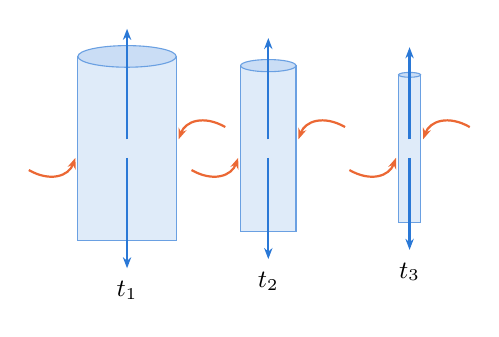
\begin{tikzpicture}[x=0.78cm, y=0.78cm, >={Stealth[length=4pt]}]
      \foreach \i/\rx/\h/\lab in {0/0.8/1.5/{$t_1$}, 1/0.45/1.35/{$t_2$}, 2/0.18/1.2/{$t_3$}} {
        \begin{scope}[shift={(\i*2.3, 0)}]
          \fill[aware!15, draw=aware!70] (-\rx, -\h) rectangle (\rx, \h);
          \draw[aware!70, fill=aware!25] (0, \h) ellipse [x radius=\rx, y radius=0.22*\rx];
          \draw[->, naive, thick] (\rx+0.8, 0.35) .. controls (\rx+0.45, 0.55) and (\rx+0.15, 0.45) .. (\rx+0.04, 0.15);
          \draw[->, naive, thick] (-\rx-0.8, -0.35) .. controls (-\rx-0.45, -0.55) and (-\rx-0.15, -0.45) .. (-\rx-0.04, -0.15);
          \draw[->, aware, thick] (0, 0.15) -- (0, \h+0.45);
          \draw[->, aware, thick] (0, -0.15) -- (0, -\h-0.45);
          \node[below, font=\small] at (0, -\h-0.5) {\lab};
        \end{scope}
      }
    \end{tikzpicture}
    \\[2pt]{\scriptsize\color{inkmuted} After Fig.\,1 of the manuscript. Orange: inward spiral; blue: outflow along the axis.}
    \column{0.58\textwidth}
    \begin{itemize}
      \item A spinning column whose radius shrinks faster than its height:
        thinner, longer, faster. OpenAI's phrase: \q{like spaghetti}.
      \item Fluid spirals in and leaves along the axis. Pulling mass inward
        speeds up the spin (the figure-skater effect). Viscosity pushes back
        and loses.
      \item Energy stays finite because the fast region shrinks faster than
        the speed grows.
      \item The catch: the force needed to hold the bare vortex together would
        itself blow up. The fix: a sequence of fine \textbf{ripples} whose own
        momentum transport cancels the bad part. What is left is a smooth force.
    \end{itemize}
  \end{columns}
  \src{Source: manuscript \S2, pp.\,3--6.}
\end{frame}

\begin{frame}{How it was produced, in OpenAI's own account}
  \begin{itemize}
    \item An internal model \q{significantly more capable than GPT-6 Astra},
      in training since 28 August.
    \item A system of \textbf{coordinating agents} with tools (a cached copy of
      the internet, code execution), split into groups that talk within the
      group. Different groups were given the four variants (A)--(D).
    \item Warm-up: the unforced Euler question fell first, to \q{nearly 100
      agents} in about 50 hours. Everything was then pointed at Navier--Stokes,
      seeded with that solution; Codex was used to cross-pollinate the groups.
    \item \q{On the order of 10,000 concurrent agents}, 88 hours, 2.7 million
      messages, about 130 billion output tokens. Lean formalization: 17 more
      hours with GPT-6 Astra.
    \item Cost: \q{millions of dollars} (Mark Chen, to \emph{Science}). Outside
      estimates run from \$1M to tens of millions. OpenAI will not claim the prize.
  \end{itemize}
  \src{Source: openai.com/index/navier-stokes-solution (8 Sep, updated 10 Sep); Science, 8 Sep. Nature and Science quote the briefing as \q{1,000 agents} for the warm-up; the post says \q{nearly 100}. A small reminder to check press numbers against the primary source.}
\end{frame}

\begin{frame}{The parallel story: a year, two people, several models}
  \begin{itemize}
    \item Tristan Buckmaster (NYU) and Levent Alpöge (Anthropic), a personal
      collaboration paid from Buckmaster's own research funds.
    \item The programme: forced-blowup constructions of Córdoba and
      Martínez-Zoroa (Madrid). Goal: push them to smooth forcing and to 3-D
      Euler. Tools: Claude and Codex (GPT-5.6 Sol; Astra for write-ups and auditing).
    \item Slow for most of a year; results on 15 August, Lean-verified 22 August.
      \q{The first LLM generated proof Levent sent me was the most horrendous I
      have ever read.}
    \item Released 7 September, earlier than planned: \q{The Euler writeup, in
      particular, can only be described as AI slop.}
    \item His framing: \q{This is a Deep Blue--Kasparov moment.}
    \item Same night, a third route: Anandkumar's group (Caltech) posted a
      numerically stable unforced-Euler blowup candidate found with a
      physics-informed neural network. Not yet a proof.
  \end{itemize}
  \src{Sources: Buckmaster's statement (cims.nyu.edu/\textasciitilde tristanb); Tao, 8 Sep; anima-ai.org, 7 Sep. Fefferman, to Quanta: \q{The heroes of the story are Córdoba and Martínez-Zoroa.}}
\end{frame}

\begin{frame}{The dispute, as each side tells it}
  \footnotesize
  \begin{columns}[t]
    \column{0.49\textwidth}
    \textbf{Buckmaster's statement (7 Sep)}
    \begin{itemize}
      \item Emailed OpenAI on 3 Sep; two calls on 6 Sep with Bubeck and an
        OpenAI mathematician. Told the proof came with \q{very little human
        input}, which \q{turned out not to be true}.
      \item \q{I asked whether the model had been trained on, or had access to,
        our sessions in Codex \ldots I asked again, about training, and I did not
        get an answer.}
      \item Two proposals, one a paper by Buckmaster alone crediting an OpenAI
        model, with Alpöge removed. Declined both. Then: \q{If you don't want
        me to be nice, then I don't have to be nice.}
      \item \q{I am not accusing anyone of anything. I am stating what I was
        told, when, and what was proposed to me.}
    \end{itemize}
    \column{0.49\textwidth}
    \textbf{OpenAI's post (8 Sep, updated 10 Sep)}
    \begin{itemize}
      \item The effort \q{began on September 1st after hearing a rumor which we
        later realized was related to} the pair.
      \item \q{We (the researchers and the agents) did not see any of their work
        through any means until they released it publicly.}
      \item 8 Sep: \q{we cannot rule out that de-identified data derived from
        their usage of our products helped improve our models.} 10 Sep, after an
        investigation: their Codex prompts \q{could not have influenced the
        system in any way, including through training.}
      \item \q{We recognize the priority of their work on forced Euler}; offered
        to show the prompts and the proof.
    \end{itemize}
  \end{columns}
  \src{Neither account is independently verified. This slide reports claims and responses, not findings.}
\end{frame}

\begin{frame}{Reactions}
  \small
  \begin{itemize}
    \item \textbf{Clay Mathematics Institute} (11 Sep): \q{apparently been
      settled}; evaluation and credit \q{deliberately unhurried}. Site status: \emph{Active}.
    \item \textbf{American Mathematical Society} (8 Sep): \q{a milestone advance
      in human knowledge}.
    \item \textbf{25 Fields Medalists} (11 Sep): \q{solving problems is only a
      tool and proxy for achieving the primary goal of conceptual understanding
      and insight}; rushed announcements raise \q{severe attribution and
      plagiarism questions}.
    \item \textbf{Terence Tao}: open problems \q{are being mined as a
      non-renewable resource}; \q{even the rumor of someone working on a problem
      can trigger a massive amount of AI-powered effort to flatten it}.
    \item \textbf{Michael Harris} (Columbia, to \emph{Science}): it \q{convinces
      decision makers that human mathematicians are obsolete}.
    \item \textbf{Sébastien Bubeck} (OpenAI): \q{the spectacular culmination of
      the arc we have seen over the last 12 months}; next, \q{developing new
      materials, finding cures to diseases}.
    \item \textbf{Nature editorial} (16 Sep): AI companies must work with the
      research community to protect attribution.
  \end{itemize}
\end{frame}

\begin{frame}{What \q{machine-checked} does and does not mean}
  \begin{columns}[t]
    \column{0.49\textwidth}
    \textbf{Lean checks}
    \begin{itemize}
      \item That every step follows from three standard axioms. No gaps, no
        \q{clearly}.
      \item Reproducibly: clone the repository, build it, run the independent
        checker.
    \end{itemize}
    \column{0.49\textwidth}
    \textbf{Humans still check}
    \begin{itemize}
      \item That the formal theorem \emph{is} the Clay statement. OpenAI
        targeted an independent transcription of it (Google DeepMind's), which
        helps. Still a judgment.
      \item Whether the construction teaches anything.
      \item Clay: publication, a two-year wait, then a committee.
    \end{itemize}
  \end{columns}
  \vspace{2pt}
  \begin{block}{Quanta, 8 Sep}
    \small\q{The crucial bit of verification that must still be done by humans is to
    guarantee that the statement being shown to be true in Lean is logically
    equivalent to what mathematicians set out to prove.}
  \end{block}
\end{frame}

\begin{frame}{Questions to argue about}
  \begin{enumerate}
    \item \textbf{Letter vs.\ spirit.} The statement allows a smooth force, and
      this result uses one. Is the Millennium problem solved?
    \item \textbf{Credit.} Córdoba and Martínez-Zoroa's ideas; Alpöge and
      Buckmaster's year; OpenAI's 88 hours. Who gets what?
    \item \textbf{Trust.} Would you put unpublished work into a frontier lab's
      tools? What would you need to see first?
    \item \textbf{Compute.} No university can run 10,000 agents for four days.
      What does that do to a field whose scarce resource was always ideas?
    \item \textbf{What is still human?} Choosing the problem, the physical
      picture, judging what matters, deciding what to formalize, and writing it
      so other people understand it.
  \end{enumerate}
\end{frame}

\section{Part 2: the other kind}

\begin{frame}{My corner of this world}
  \begin{itemize}
    \item 2016 PhD, applied mathematics, CU Boulder: simulating waves
      travelling through \textbf{layered materials}. Seismic imaging (sound
      through rock), ultrasound (sound through tissue).
    \item The contribution: \q{interface-aware} stencils, that is,
      simulation building blocks that know where the material changes.
    \item Written in MATLAB, nine years ago. I no longer have a licence, and
      the code was never meant for anyone else to read.
    \item The experiment: with Claude Code, re-derive the method from the
      papers, port it to Python, and verify it against exact solutions.
    \item Result: the 1-D method and the 2-D method, both working and tested,
      in one day.
  \end{itemize}
\end{frame}

\begin{frame}{The problem in one picture}
  \begin{columns}[c]
    \column{0.5\textwidth}
    \centering
    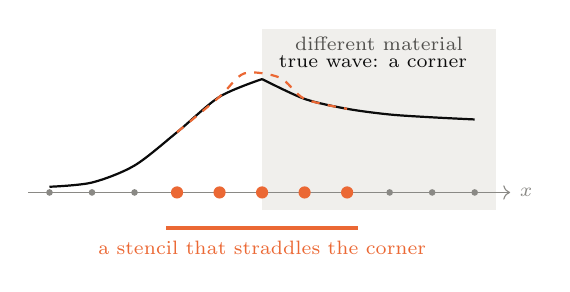
\begin{tikzpicture}[x=0.9cm, y=0.9cm]
      \fill[layer] (0, -0.25) rectangle (3.3, 2.3);
      \node[font=\scriptsize, inksec] at (1.65, 2.1) {different material};
      \draw[->, inkmuted] (-3.3, 0) -- (3.5, 0) node[right, font=\scriptsize] {$x$};
      \draw[thick, ink] plot[smooth] coordinates {(-3, 0.08) (-2.4, 0.14) (-1.8, 0.38) (-1.2, 0.85) (-0.6, 1.35) (0, 1.6)};
      \draw[thick, ink] plot[smooth] coordinates {(0, 1.6) (0.6, 1.32) (1.2, 1.18) (1.8, 1.1) (2.4, 1.06) (3, 1.03)};
      \foreach \x in {-3, -2.4, ..., 3.01} {\fill[inkmuted] (\x, 0) circle (1.2pt);}
      \draw[naive, dashed, thick] plot[smooth] coordinates {(-1.2, 0.85) (-0.6, 1.35) (-0.25, 1.68) (0.25, 1.62) (0.6, 1.32) (1.2, 1.18)};
      \foreach \x in {-1.2, -0.6, 0, 0.6, 1.2} {\fill[naive] (\x, 0) circle (2.2pt);}
      \draw[naive, very thick] (-1.35, -0.5) -- (1.35, -0.5);
      \node[naive, font=\scriptsize, below] at (0, -0.55) {a stencil that straddles the corner};
      \node[ink, font=\scriptsize, above right] at (0.1, 1.62) {true wave: a corner};
    \end{tikzpicture}
    \column{0.5\textwidth}
    \begin{itemize}
      \item A simulation stores the wave at grid points and estimates slopes
        from a few neighbours: a \textbf{stencil}.
      \item Where the material changes, the wave is continuous but its
        \emph{slope jumps}: a corner.
      \item A stencil straddling the corner assumes a smooth wave (dashed) and
        gets the slope wrong. The error shows up as ringing and wrong reflections.
      \item The fix: rebuild the handful of stencils near the boundary from
        pieces that obey the jump conditions. Everything else is unchanged.
    \end{itemize}
  \end{columns}
\end{frame}

\begin{frame}{1-D: the ringing, and the fix}
  \begin{columns}[c]
    \column{0.56\textwidth}
    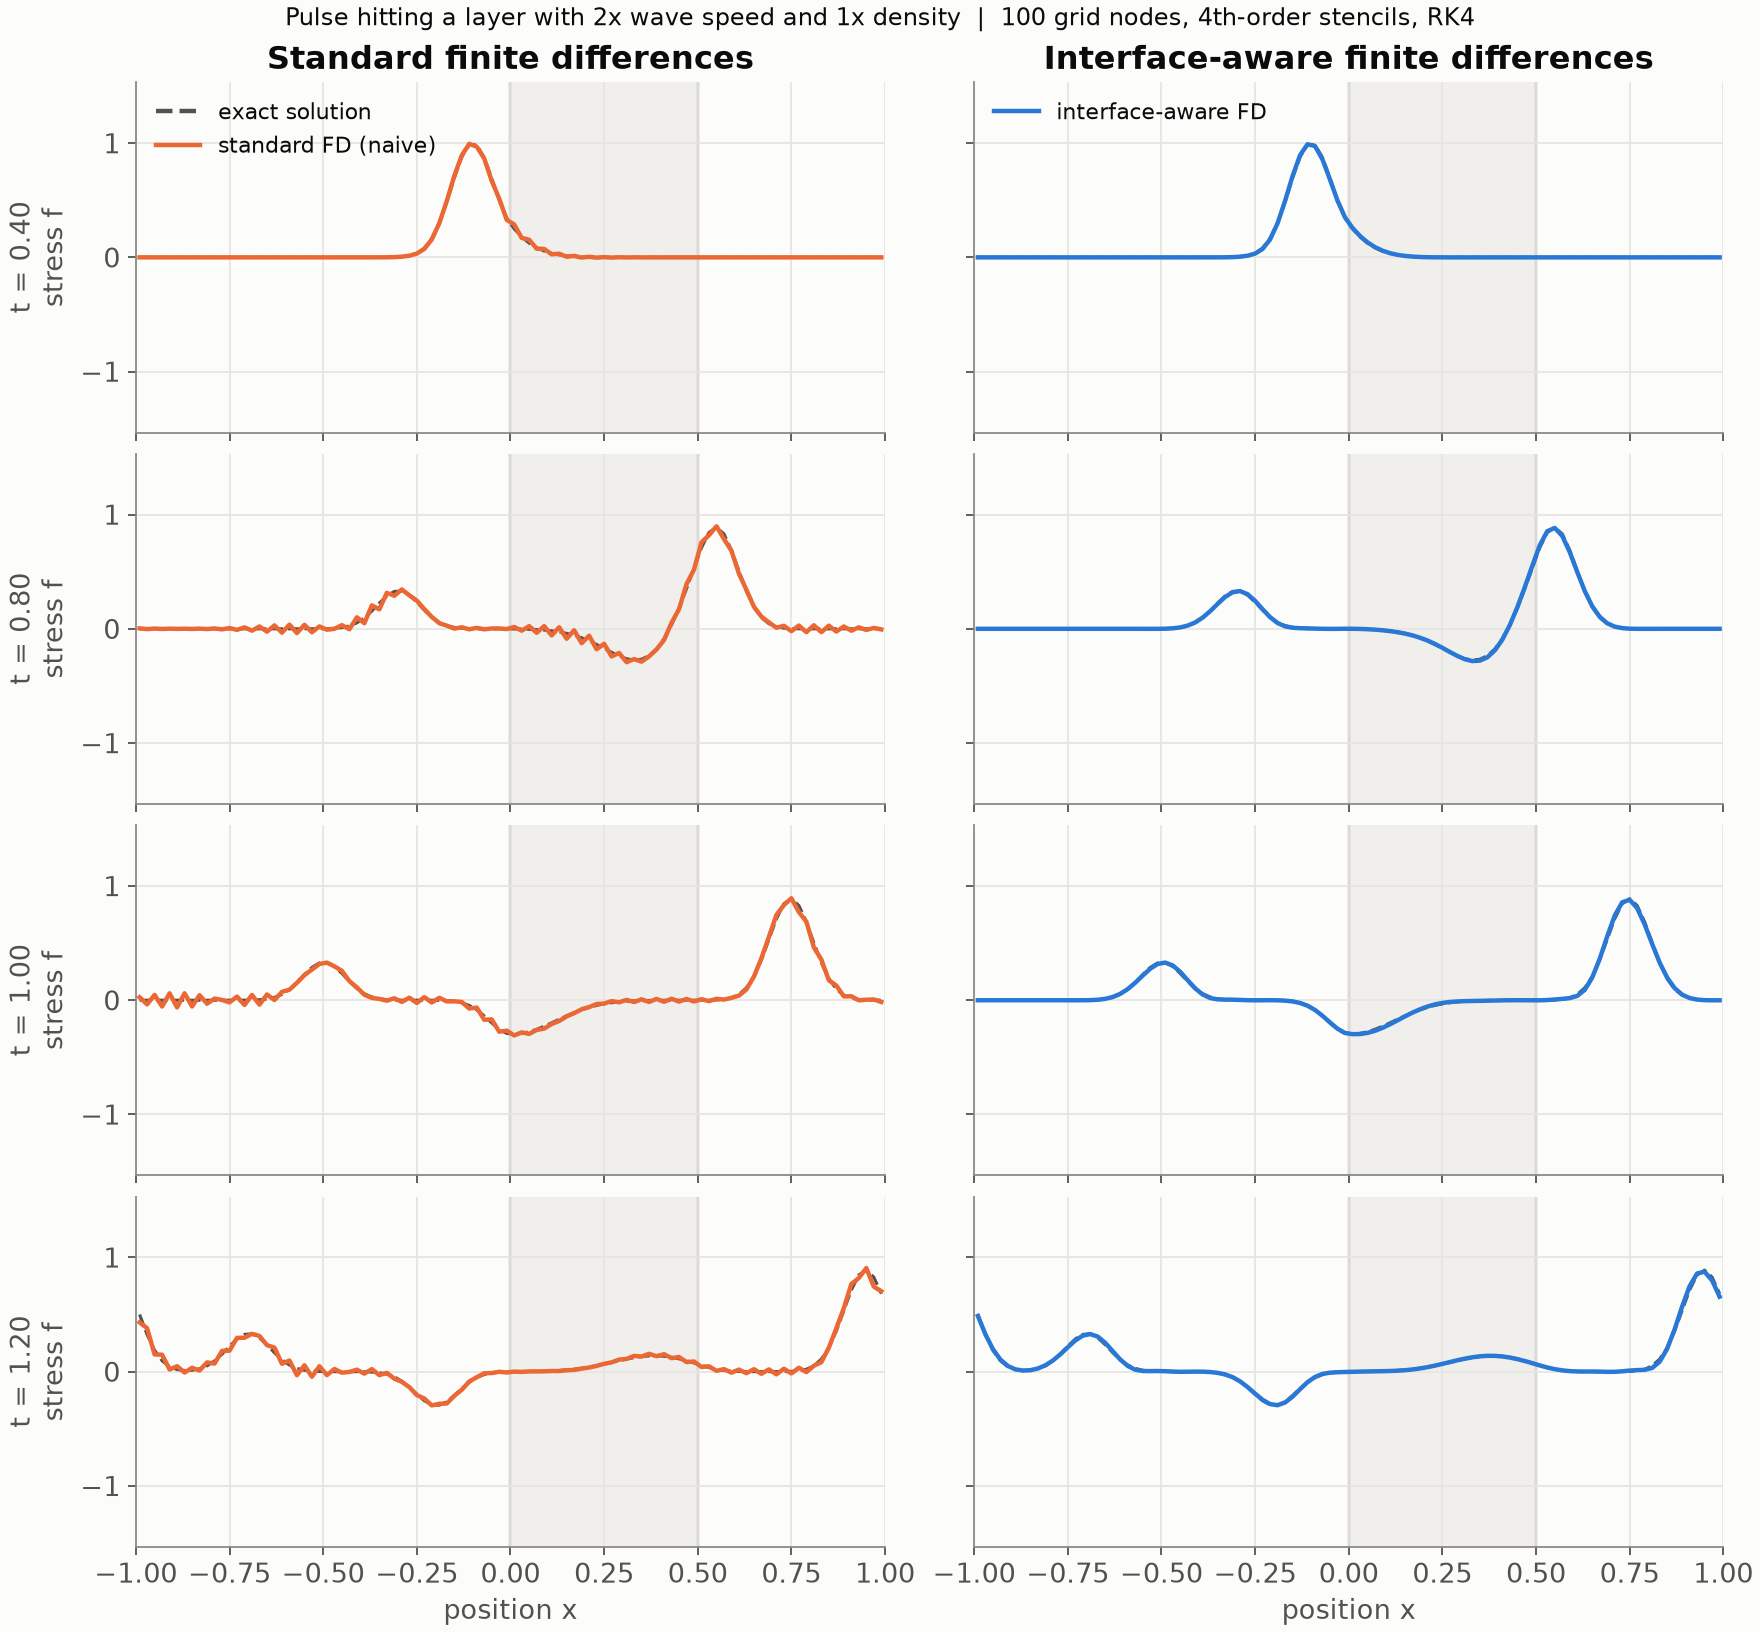
\includegraphics[height=0.8\textheight]{figures/wave1d_naive_vs_aware_coarse.png}
    \column{0.42\textwidth}
    \small
    \begin{itemize}
      \item A pulse hits a layer (shaded) where waves travel twice as fast.
        Part reflects, part transmits.
      \item Both panels: 100 grid points, the same time step, the same code.
        Only the stencils touching the layer edges differ.
      \item \textcolor{naive}{Standard}: a trail of wiggles behind every
        reflection; 10\% error by $t = 1$.
        \textcolor{aware}{Interface-aware}: on the exact solution; 3\% error,
        all of it from the coarse grid.
    \end{itemize}
    \clipnote{wave1d\_naive\_vs\_aware\_coarse.mp4}{10 s}
  \end{columns}
\end{frame}

\begin{frame}{1-D: how fast the error shrinks}
  \centering
  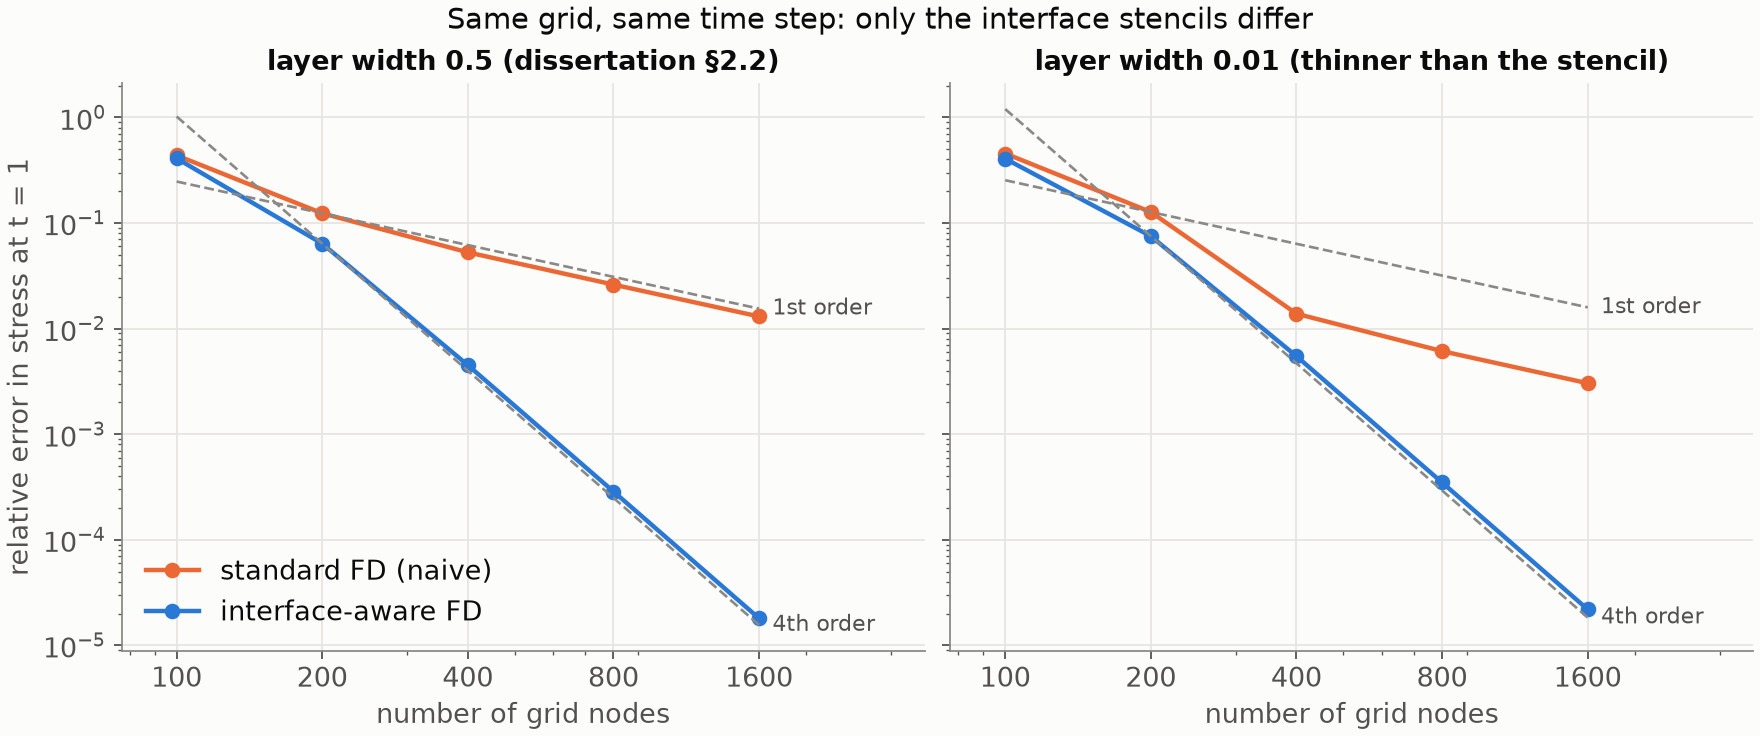
\includegraphics[width=0.74\textwidth]{figures/wave1d_convergence.png}
  \begin{itemize}
    \item \textcolor{naive}{Standard}: double the points, halve the error
      (\q{first order}). The corner caps the accuracy however good the stencils
      are elsewhere.
    \item \textcolor{aware}{Interface-aware}: double the points, divide the
      error by 16 (\q{fourth order}). Also for a layer thinner than the stencil (right).
  \end{itemize}
  \src{Reproduces Fig.\,2-8 of the dissertation. Error measured against an exact ray-sum solution at $t = 1$.}
\end{frame}

\begin{frame}{2-D: scattered points and curved boundaries}
  \centering
  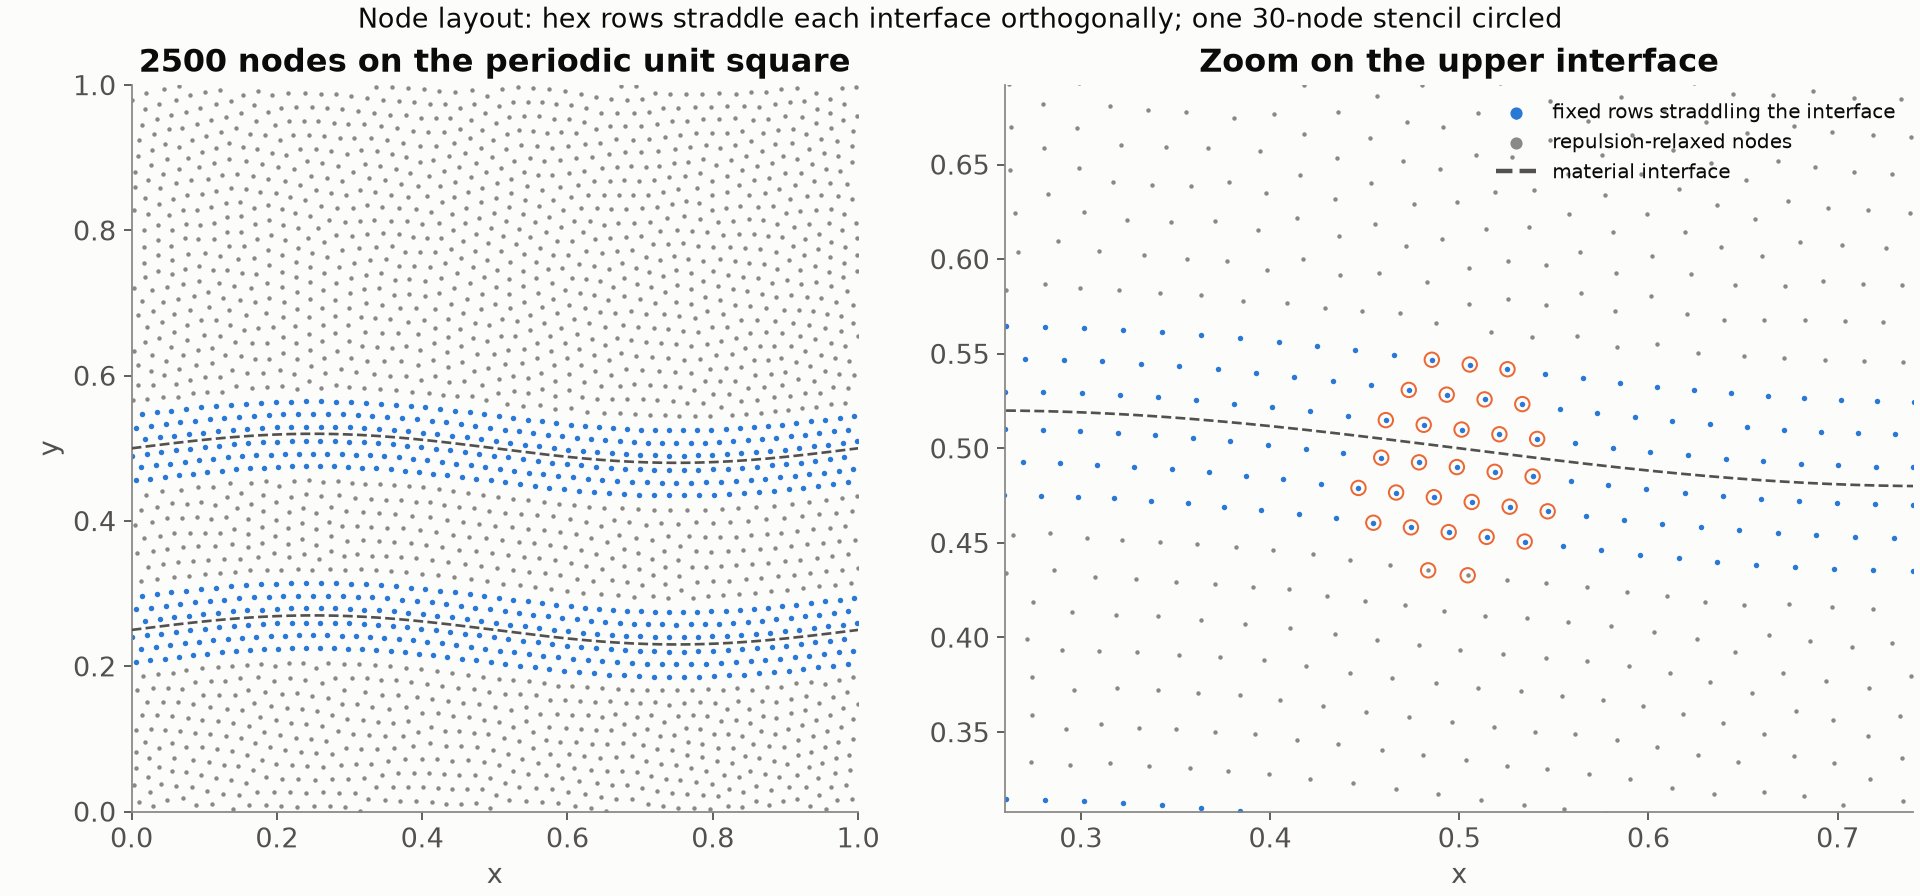
\includegraphics[width=0.66\textwidth]{figures/wave2d_nodes.png}
  \begin{itemize}
    \item No grid. Points are spread by a repulsion process, with fixed rows
      straddling each boundary (blue). That layout was the key to stability; it
      took years to find and is still unproven.
    \item Each point's stencil is its 30 nearest neighbours, weighted with radial
      basis functions plus polynomials (RBF-FD). Five fields: two velocities,
      three stresses.
  \end{itemize}
\end{frame}

\begin{frame}{2-D: same points, only the stencils near the boundaries differ}
  \begin{columns}[c]
    \column{0.58\textwidth}
    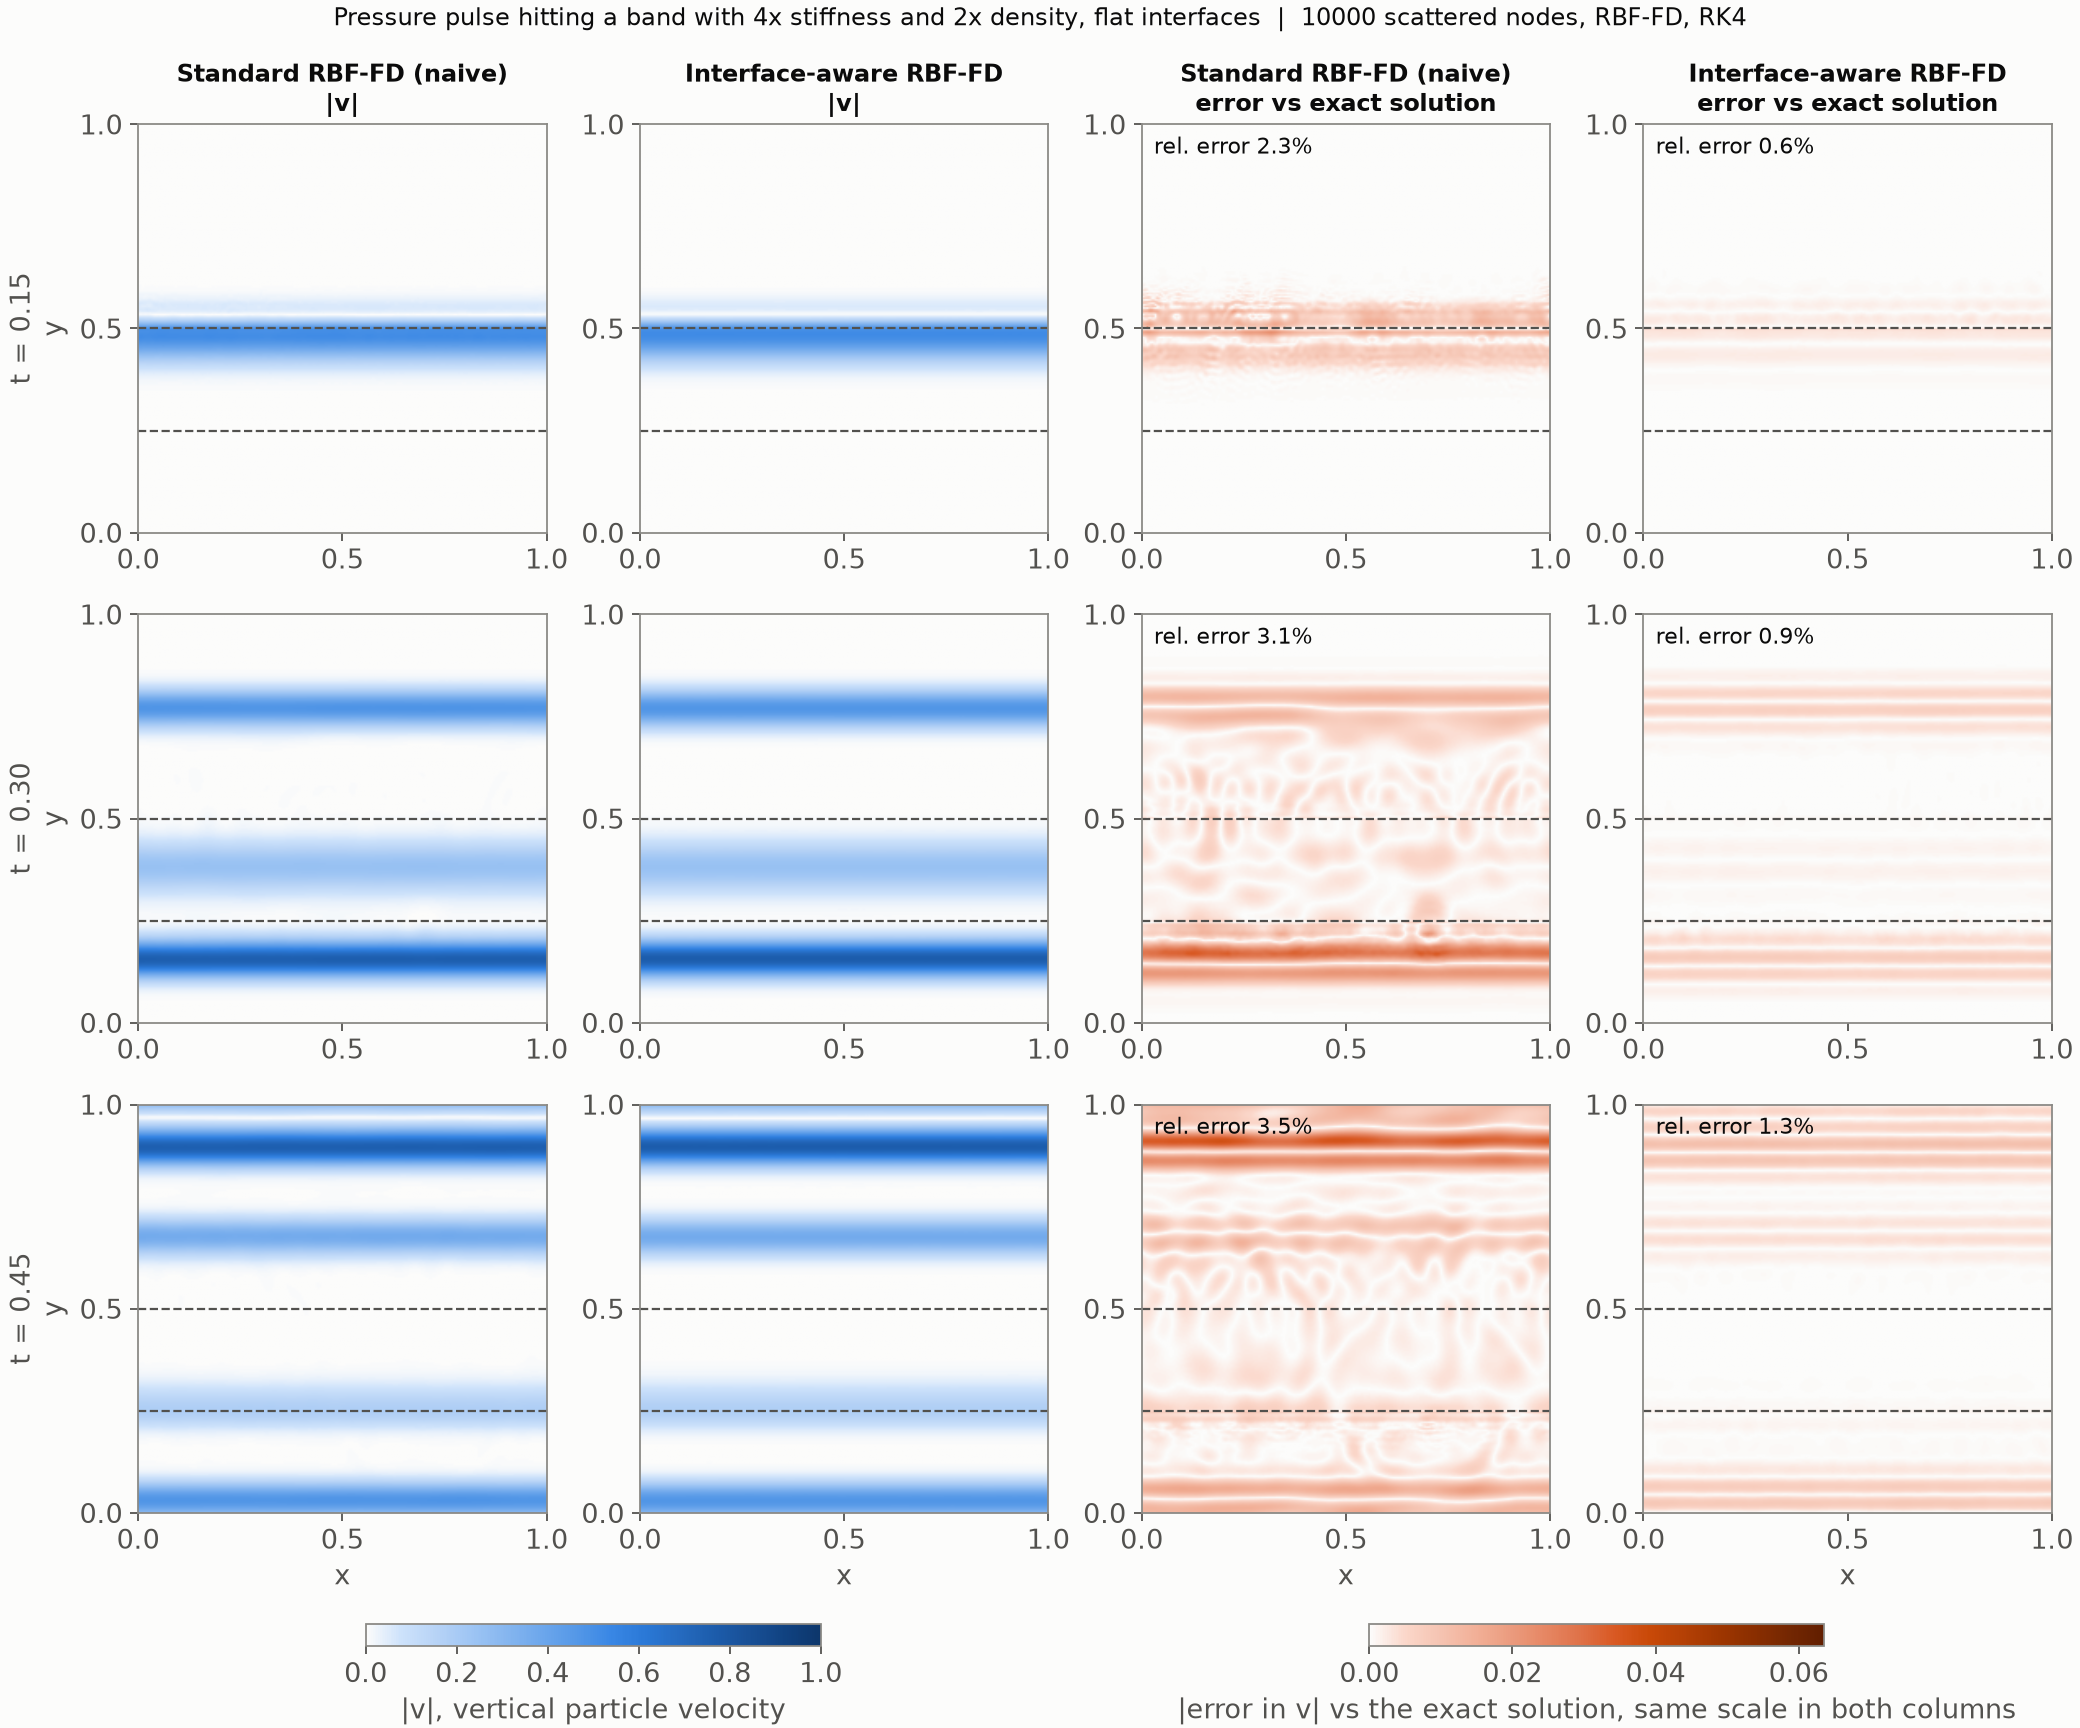
\includegraphics[height=0.8\textheight]{figures/wave2d_naive_vs_aware.png}
    \column{0.4\textwidth}
    \small
    \begin{itemize}
      \item A pressure pulse travels down through a band of stiffer, denser
        material. 10,000 points.
      \item Left pair: the wave. Right pair: the error against the exact
        solution, on one colour scale.
      \item At $t = 0.3$: \textcolor{naive}{standard} 3.1\% error,
        \textcolor{aware}{interface-aware} 0.9\%. The standard error starts at
        the boundary, then travels with the wave.
    \end{itemize}
    \clipnote{wave2d\_naive\_vs\_aware.mp4, then \_curved.mp4}{8 s each}
  \end{columns}
\end{frame}

\begin{frame}{2-D: the boundary error is gone}
  \centering
  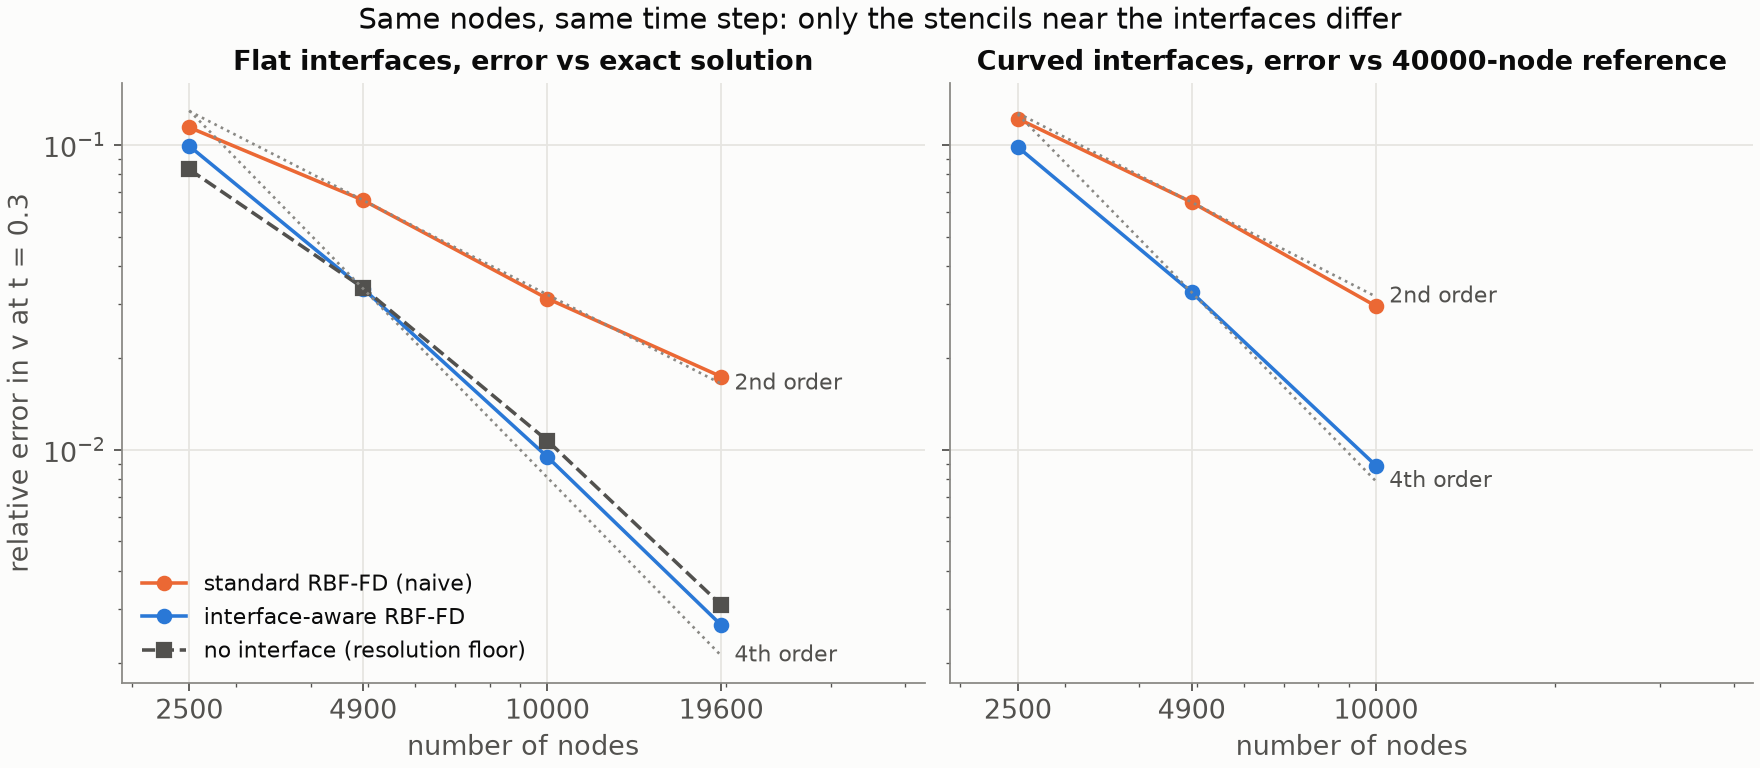
\includegraphics[width=0.66\textwidth]{figures/wave2d_convergence.png}
  \begin{itemize}
    \item Dashed: the same pulse in a uniform material, so pure resolution error
      with no boundary at all.
    \item The \textcolor{aware}{interface-aware} error sits on that floor: at
      these resolutions there is nothing left to fix at the boundary. Curved
      boundaries (right) give the same numbers.
  \end{itemize}
  \src{Reproduces Fig.\,3-5 and 3-8 of the dissertation. Left: error against the exact solution. Right: against a 40,000-point reference run.}
\end{frame}

\begin{frame}{What the collaboration looked like}
  \begin{columns}[t]
    \column{0.5\textwidth}
    \textbf{One day (17 Sep)}
    \begin{itemize}
      \item 8 issues, 7 pull requests, 26 commits, 106 tests, all green.
      \item Every numerical routine tested against an exact solution or a
        convergence rate, not \q{it runs}.
      \item Independent reference solutions built before trusting a solver.
      \item Adversarial review passes caught three real bugs: a sign error, two
        latent bugs in the exact solver that only the 2-D problem exposed, a
        crash in a driver.
    \end{itemize}
    \column{0.5\textwidth}
    \textbf{What was still human}
    \begin{itemize}
      \item Where to put the points (the straddling rows).
      \item Plain method first, clever method second.
      \item Which basis functions, and the narrow window for the stabilising
        parameter.
      \item \q{Don't let the error measurement itself cross a boundary.}
      \item Same list as Part 1: steering, judging what matters, designing the
        verification. The typing, the bookkeeping, and the port were not.
    \end{itemize}
  \end{columns}
\end{frame}

\begin{frame}{Two kinds of AI in research math}
  \footnotesize
  \begin{tabular}{@{}lp{3.4cm}p{3.4cm}p{3.4cm}@{}}
    \toprule
     & OpenAI, Navier--Stokes & Alpöge and Buckmaster & This afternoon \\
    \midrule
    Who steered & a lab team, via prompts & two mathematicians & one engineer \\
    Scale & $\sim$10,000 agents, 88 h & about a year, several models & one assistant, one day \\
    Verification & Lean; Clay review pending & Lean; papers being rewritten & tests against exact solutions \\
    Who understands it & contested & \q{AI slop}, being digested & fully; it is my method \\
    Cost & millions of dollars & own research funds & a subscription \\
    \bottomrule
  \end{tabular}
  \vspace{10pt}
  \normalsize
  \begin{itemize}
    \item The capability is real at both ends of this table.
    \item The difference is who steered, who can check it, and who is left
      understanding the result.
  \end{itemize}
\end{frame}

\begin{frame}{For the curious}
  \footnotesize
  \textbf{Gentle starts}
  \begin{itemize}
    \item 3Blue1Brown, \href{https://www.youtube.com/watch?v=ly4S0oi3Yz8}{\emph{But what is a partial differential equation?}} (YouTube, 17 min)
    \item Khan Academy: \href{https://www.khanacademy.org/math/differential-equations}{Differential equations};
      \href{https://www.khanacademy.org/math/multivariable-calculus/multivariable-derivatives/partial-derivative-and-gradient-articles/a/introduction-to-partial-derivatives}{Introduction to partial derivatives}
    \item Wikipedia: \href{https://en.wikipedia.org/wiki/Navier\%E2\%80\%93Stokes_existence_and_smoothness}{Navier--Stokes existence and smoothness};
      \href{https://en.wikipedia.org/wiki/Finite_difference_method}{Finite difference method};
      \href{https://en.wikipedia.org/wiki/Lean_(proof_assistant)}{Lean (proof assistant)}
  \end{itemize}
  \textbf{Primary sources for Part 1}
  \begin{itemize}
    \item OpenAI: \href{https://openai.com/index/navier-stokes-solution/}{the announcement and manuscript}; \href{https://github.com/openai/NavierStokesAndEuler}{the Lean repository}
    \item Clay Mathematics Institute: \href{https://www.claymath.org/millennium/navier-stokes-equation/}{the problem page and official statement}
    \item \href{https://cims.nyu.edu/~tristanb/statement.pdf}{Buckmaster's statement} and papers (cims.nyu.edu/\textasciitilde tristanb)
    \item \href{https://terrytao.wordpress.com/2026/09/07/finite-time-blowup-with-smooth-forcing-term-for-the-incompressible-porous-medium-boussinesq-and-incompressible-euler-equations/}{Tao's blog post, 7 Sep 2026}; \href{https://mathandai.org/}{the Fields Medalists' declaration}
  \end{itemize}
  \textbf{Part 2}
  \begin{itemize}
    \item Code, tests, figures, and these notes: \href{https://github.com/bradleypmartin/20260930-zd-ai-pdes-demo}{github.com/bradleypmartin/20260930-zd-ai-pdes-demo} (MIT)
  \end{itemize}
\end{frame}

\appendix

\begin{frame}{Backup: the equations}
  For velocity $u(x,t)$, pressure $p(x,t)$, viscosity $\nu > 0$, and force $f$:
  \[
    \partial_t u + (u \cdot \nabla) u - \nu \Delta u + \nabla p = f,
    \qquad \nabla \cdot u = 0 .
  \]
  \begin{itemize}
    \item Left to right: acceleration, transport by the flow itself (the
      nonlinear term, and the source of all the difficulty), viscous
      smoothing, pressure. Right: the stirring force.
    \item Second equation: the fluid is incompressible.
    \item Theorem 1.1: for every $\nu > 0$ there are a smooth compactly
      supported $f$ and smooth $(u, p)$ on $\mathbb{R}^3 \times [0, 1)$ with
      $u(\cdot, 0) = 0$, $\sup_t \|u(t)\|_{L^2} < \infty$, and
      $\limsup_{t \uparrow 1} \|u(t)\|_{L^\infty} = \infty$.
  \end{itemize}
\end{frame}

\begin{frame}{Backup: keeping the 2-D method stable}
  \centering
  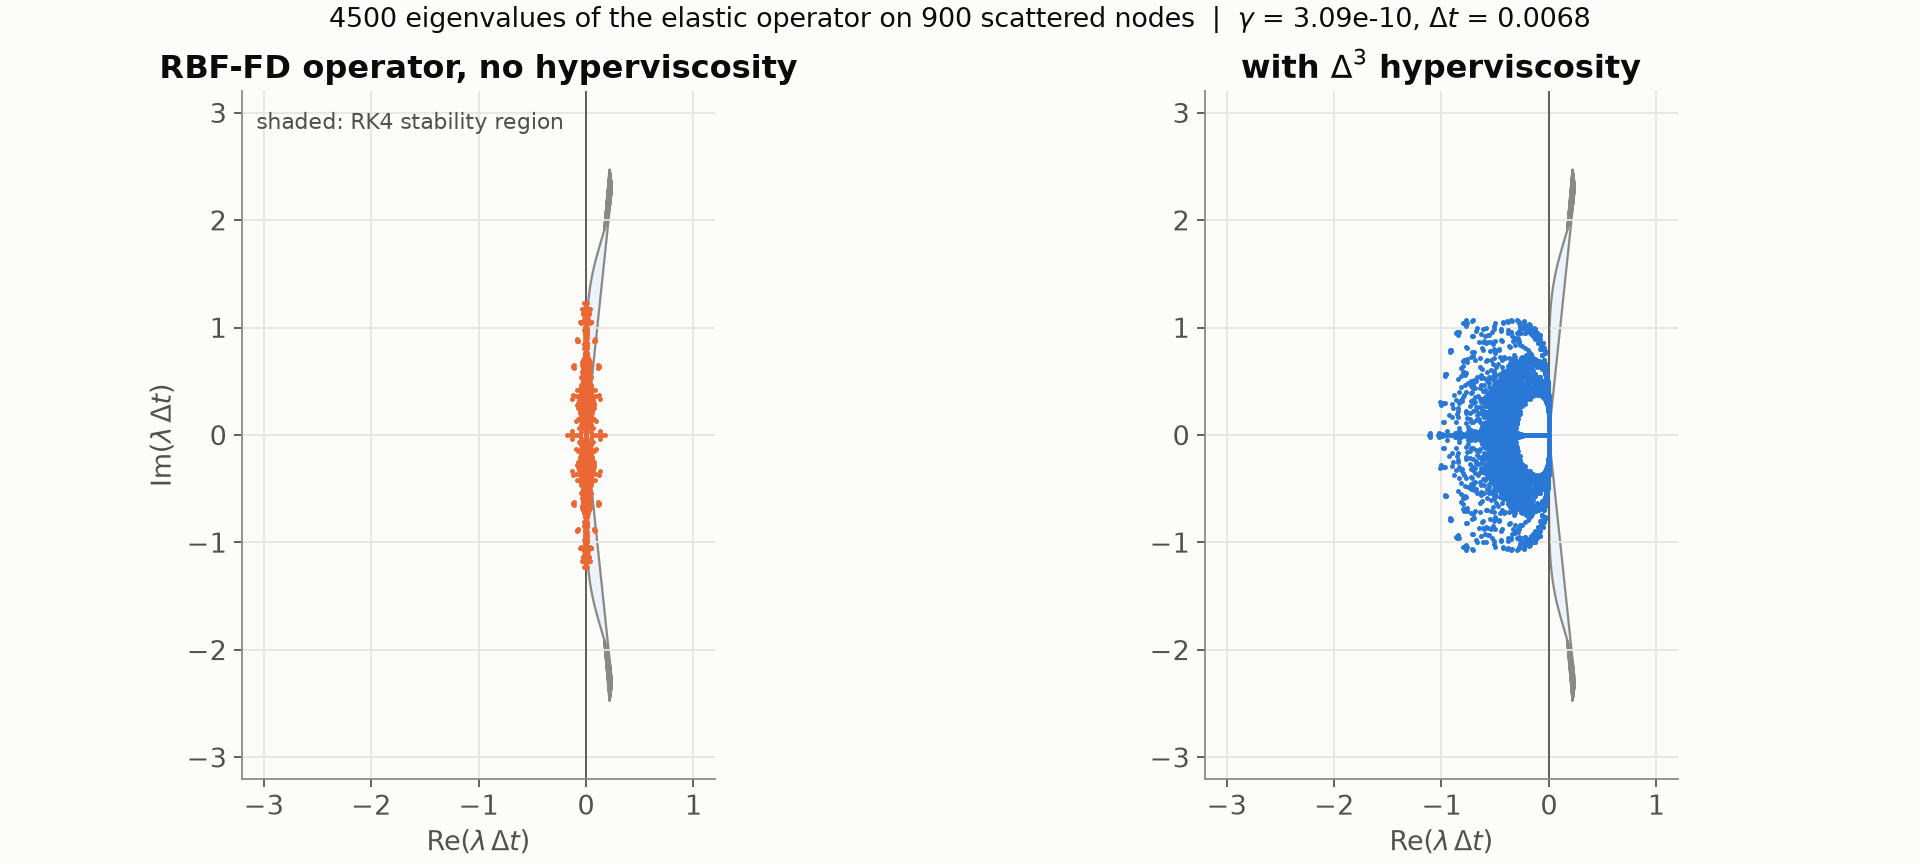
\includegraphics[width=0.7\textwidth]{figures/wave2d_eigenvalues.png}
  \begin{itemize}
    \item Scattered-point stencils leave a few growing modes (left, orange
      outside the stability region). A small high-order damping term
      (\q{hyperviscosity}) moves them inside (right) without touching the
      accurate ones.
    \item Its size has to scale with the point spacing in a narrow window. That
      window was a human input; the eigenvalue check was the assistant's.
  \end{itemize}
\end{frame}

\begin{frame}{Backup: Part 2 numbers}
  \small
  \begin{columns}[t]
    \column{0.48\textwidth}
    \textbf{1-D, relative error in stress at $t = 1$}
    \begin{tabular}{@{}rrr@{}}
      \toprule
      points & standard & interface-aware \\
      \midrule
      200 & $1.2\times10^{-1}$ & $6.4\times10^{-2}$ \\
      400 & $5.3\times10^{-2}$ & $4.5\times10^{-3}$ \\
      800 & $2.6\times10^{-2}$ & $2.9\times10^{-4}$ \\
      1600 & $1.3\times10^{-2}$ & $1.8\times10^{-5}$ \\
      \bottomrule
    \end{tabular}
    \column{0.48\textwidth}
    \textbf{2-D, flat boundaries, error in $v$ at $t = 0.3$}
    \begin{tabular}{@{}rrrr@{}}
      \toprule
      points & standard & aware & no boundary \\
      \midrule
      2500 & $1.1\times10^{-1}$ & $9.9\times10^{-2}$ & $8.2\times10^{-2}$ \\
      4900 & $6.9\times10^{-2}$ & $3.4\times10^{-2}$ & $3.3\times10^{-2}$ \\
      10000 & $3.1\times10^{-2}$ & $9.6\times10^{-3}$ & $1.1\times10^{-2}$ \\
      19600 & $1.7\times10^{-2}$ & $2.7\times10^{-3}$ & $3.0\times10^{-3}$ \\
      \bottomrule
    \end{tabular}
  \end{columns}
  \vspace{6pt}
  \src{From docs/demo-outline.md; drivers scripts/wave1d\_convergence.py and scripts/wave2d\_convergence.py.}
\end{frame}

\end{document}
